\section*{\nr.3 \titthree (25 Punkte)}
\begin{enumerate}[(a)]
\item Sein $N_\gamma$ die Anzahl von Photonen mit Frequenz $\nu$, die in einem bestimmten Zeitraum auf die Solarzelle treffen. Diese bringen eine Energie von
\begin{equation}
E = h \nu N_\gamma
\end{equation}
mit. Durch die Absorption durch die Solarzelle werden statistisch $\eta N_\gamma$ Elektronen aus ihrem Gitter gelöst, wobei $\eta$ die Quanteneffizienz bezeichnet. Die betragsmäßige Ladung eines Elektrons beträgt eine Elementarladung $e$, sodass die Gesamtladung
\begin{equation}
Q = \eta N_\gamma e
\end{equation} 
im betrachteten Zeitpunkt herausgeschlagen wird.
Für die Responsivität folgt mit $c=\lambda \nu$:
\begin{equation}
R = \frac{Q}{E} = \frac{\eta N_\gamma e}{h \nu N_\gamma} = \frac{\eta e}{h \nu} = \frac{\eta e}{hc} \lambda
\end{equation}
So ergibt sich der in der Abbildung zu erklärende proportionale Zusammenhang zwischen Responsivität und Wellenlänge. Solarzellen sind effizient gebaut, sodass uns vernünftig erschien, die Quanteneffizienz in den folgenden Rechnungen auf $\eta = 1$ zu setzen. So ergibt sich für die Steigung des idealisierten Verlaufs ein Wert von ca. \SI{8e5}{\ampere\per\watt\per\meter}, der sich mit dem Wert deckt, den man durch graphisches Ablesen der Steigung erhält.
\item Eine Skizze der spektralen Strahlungsleistung der Sonne pro Fläche ist durch \vref{fig:sonnenspektrum} gegeben.
\begin{figure}[htbp]
\centering
% GNUPLOT: LaTeX picture with Postscript
\begingroup
  \makeatletter
  \providecommand\color[2][]{%
    \GenericError{(gnuplot) \space\space\space\@spaces}{%
      Package color not loaded in conjunction with
      terminal option `colourtext'%
    }{See the gnuplot documentation for explanation.%
    }{Either use 'blacktext' in gnuplot or load the package
      color.sty in LaTeX.}%
    \renewcommand\color[2][]{}%
  }%
  \providecommand\includegraphics[2][]{%
    \GenericError{(gnuplot) \space\space\space\@spaces}{%
      Package graphicx or graphics not loaded%
    }{See the gnuplot documentation for explanation.%
    }{The gnuplot epslatex terminal needs graphicx.sty or graphics.sty.}%
    \renewcommand\includegraphics[2][]{}%
  }%
  \providecommand\rotatebox[2]{#2}%
  \@ifundefined{ifGPcolor}{%
    \newif\ifGPcolor
    \GPcolortrue
  }{}%
  \@ifundefined{ifGPblacktext}{%
    \newif\ifGPblacktext
    \GPblacktextfalse
  }{}%
  % define a \g@addto@macro without @ in the name:
  \let\gplgaddtomacro\g@addto@macro
  % define empty templates for all commands taking text:
  \gdef\gplbacktext{}%
  \gdef\gplfronttext{}%
  \makeatother
  \ifGPblacktext
    % no textcolor at all
    \def\colorrgb#1{}%
    \def\colorgray#1{}%
  \else
    % gray or color?
    \ifGPcolor
      \def\colorrgb#1{\color[rgb]{#1}}%
      \def\colorgray#1{\color[gray]{#1}}%
      \expandafter\def\csname LTw\endcsname{\color{white}}%
      \expandafter\def\csname LTb\endcsname{\color{black}}%
      \expandafter\def\csname LTa\endcsname{\color{black}}%
      \expandafter\def\csname LT0\endcsname{\color[rgb]{1,0,0}}%
      \expandafter\def\csname LT1\endcsname{\color[rgb]{0,1,0}}%
      \expandafter\def\csname LT2\endcsname{\color[rgb]{0,0,1}}%
      \expandafter\def\csname LT3\endcsname{\color[rgb]{1,0,1}}%
      \expandafter\def\csname LT4\endcsname{\color[rgb]{0,1,1}}%
      \expandafter\def\csname LT5\endcsname{\color[rgb]{1,1,0}}%
      \expandafter\def\csname LT6\endcsname{\color[rgb]{0,0,0}}%
      \expandafter\def\csname LT7\endcsname{\color[rgb]{1,0.3,0}}%
      \expandafter\def\csname LT8\endcsname{\color[rgb]{0.5,0.5,0.5}}%
    \else
      % gray
      \def\colorrgb#1{\color{black}}%
      \def\colorgray#1{\color[gray]{#1}}%
      \expandafter\def\csname LTw\endcsname{\color{white}}%
      \expandafter\def\csname LTb\endcsname{\color{black}}%
      \expandafter\def\csname LTa\endcsname{\color{black}}%
      \expandafter\def\csname LT0\endcsname{\color{black}}%
      \expandafter\def\csname LT1\endcsname{\color{black}}%
      \expandafter\def\csname LT2\endcsname{\color{black}}%
      \expandafter\def\csname LT3\endcsname{\color{black}}%
      \expandafter\def\csname LT4\endcsname{\color{black}}%
      \expandafter\def\csname LT5\endcsname{\color{black}}%
      \expandafter\def\csname LT6\endcsname{\color{black}}%
      \expandafter\def\csname LT7\endcsname{\color{black}}%
      \expandafter\def\csname LT8\endcsname{\color{black}}%
    \fi
  \fi
    \setlength{\unitlength}{0.0500bp}%
    \ifx\gptboxheight\undefined%
      \newlength{\gptboxheight}%
      \newlength{\gptboxwidth}%
      \newsavebox{\gptboxtext}%
    \fi%
    \setlength{\fboxrule}{0.5pt}%
    \setlength{\fboxsep}{1pt}%
\begin{picture}(7936.00,5102.00)%
    \gplgaddtomacro\gplbacktext{%
      \csname LTb\endcsname%
      \put(682,704){\makebox(0,0)[r]{\strut{}$0$}}%
      \put(682,1531){\makebox(0,0)[r]{\strut{}$20$}}%
      \put(682,2357){\makebox(0,0)[r]{\strut{}$40$}}%
      \put(682,3184){\makebox(0,0)[r]{\strut{}$60$}}%
      \put(682,4010){\makebox(0,0)[r]{\strut{}$80$}}%
      \put(814,484){\makebox(0,0){\strut{}$0$}}%
      \put(2159,484){\makebox(0,0){\strut{}$200$}}%
      \put(3504,484){\makebox(0,0){\strut{}$400$}}%
      \put(4849,484){\makebox(0,0){\strut{}$600$}}%
      \put(6194,484){\makebox(0,0){\strut{}$800$}}%
    }%
    \gplgaddtomacro\gplfronttext{%
      \csname LTb\endcsname%
      \put(176,2770){\rotatebox{-270}{\makebox(0,0){\strut{}spektrale Strahlungsleistung in \si{\tera\watt\per\meter\cubed}}}}%
      \put(4176,154){\makebox(0,0){\strut{}$\lambda$ in \si{\nano\meter}}}%
    }%
    \gplgaddtomacro\gplbacktext{%
      \csname LTb\endcsname%
      \put(682,704){\makebox(0,0)[r]{\strut{}$0$}}%
      \put(682,1531){\makebox(0,0)[r]{\strut{}$20$}}%
      \put(682,2357){\makebox(0,0)[r]{\strut{}$40$}}%
      \put(682,3184){\makebox(0,0)[r]{\strut{}$60$}}%
      \put(682,4010){\makebox(0,0)[r]{\strut{}$80$}}%
      \put(814,484){\makebox(0,0){\strut{}$0$}}%
      \put(2159,484){\makebox(0,0){\strut{}$200$}}%
      \put(3504,484){\makebox(0,0){\strut{}$400$}}%
      \put(4849,484){\makebox(0,0){\strut{}$600$}}%
      \put(6194,484){\makebox(0,0){\strut{}$800$}}%
    }%
    \gplgaddtomacro\gplfronttext{%
      \csname LTb\endcsname%
      \put(176,2770){\rotatebox{-270}{\makebox(0,0){\strut{}spektrale Strahlungsleistung in \si{\tera\watt\per\meter\cubed}}}}%
      \put(4176,154){\makebox(0,0){\strut{}$\lambda$ in \si{\nano\meter}}}%
    }%
    \gplbacktext
    \put(0,0){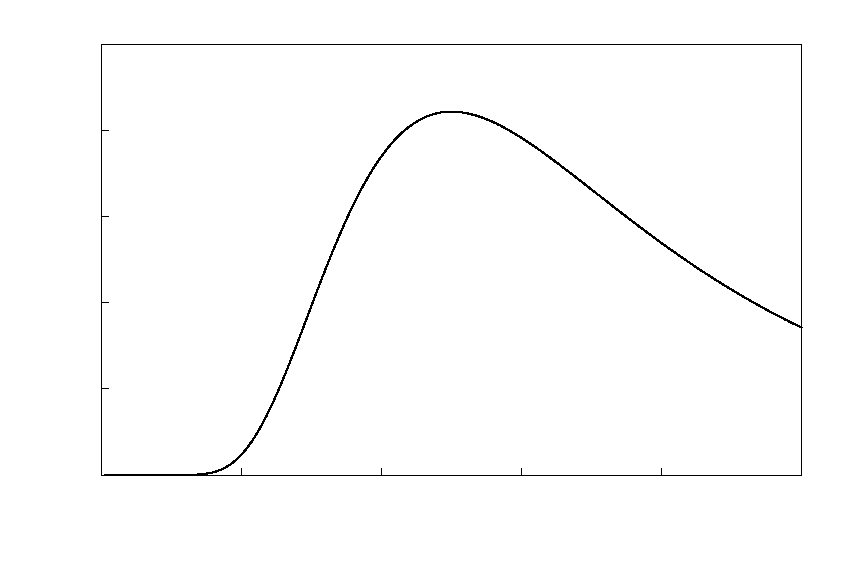
\includegraphics{sonnenspektrum}}%
    \gplfronttext
  \end{picture}%
\endgroup

\caption{Spektrale Strahlungsleistung der Sonne.}
\label{fig:sonnenspektrum}
\end{figure}

\item Sei $u(\lambda)$ die spektrale Energiedichte nach Planck. Licht eines Wellenlängenbereichs $\mathrm{d}\lambda$ strahlt im Abstand $d$ von der Sonne mit Radius $R_s$ mit einer Strahlungsleistung $\mathrm{d}S$ pro Fläche von
\begin{equation}
\mathrm{d}S = \frac{c}{4} u(\lambda) \mathrm{d}\lambda \cdot \frac{4\pi R_s^2}{4\pi d^2},
\end{equation}
wobei der Vorfaktor $c/4$ aus dem Lambertschen Gesetz folgt und auf dem letzten Zettel hergeleitet wurde. Dieses Strahlungsdifferential führt zu einem kleinen Strom von:
\begin{equation}
\mathrm{d} I_{pv} = A R \mathrm{d}S = \frac{2\pi c \eta e A \,\mathrm{d}\lambda}{\lambda^4\left\{\exp\left[hc/(\lambda k T)\right]-1 \right\}} \cdot \frac{R_s^2}{d^2}
\end{equation}
Der Gesamtstrom ergibt sich durch Integration über einen Wellenlängenbereich $\left[\lambda_\text{min}, \lambda_\text{max} \right]$:
\begin{equation}
I_{pv} = \int_{\lambda_\text{min}}^{\lambda_\text{max}}\mathrm{d} I_{pv}
\end{equation}
Aus der Abbildung ergibt sich ein vernünftiger Wellenlängenbereich von $\left[\SI{400}{\nano\meter}, \SI{1000}{\nano\meter} \right]$, in dem die Responsivität ideal ist. Außerhalb ist sie näherungsweise null. Numerische Integration mit Python liefert $I_{pv}=\SI{4.38}{\ampere}$.  
\end{enumerate}